%%%%%%%%%%%%%%%%%%%%%%%%%%%%%%%%%%%%%%%%%%%%%%%%%%%%%%%%%%%%%%%%%%
%% Scribe Editors: 
%%    - Jimmy Lin <jimmy@utexas.edu>
%%    - Vutha Va <vutha.va@utexas.edu>
%%    - David Inouye <davidinouye@gmail.com>
%%%%%%%%%%%%%%%%%%%%%%%%%%%%%%%%%%%%%%%%%%%%%%%%%%%%%%%%%%%%%%%%%%
%% The main content of LECTURE 07 contains THREE SECTIONS. 
%% Specifically,
%%    ONE: definition and interpretations of Newton Method
%%    TWO: Affine Invariance of Newton Method
%%    THREE: Convergence Analysis of Newton Method
%%%%%%%%%%%%%%%%%%%%%%%%%%%%%%%%%%%%%%%%%%%%%%%%%%%%%%%%%%%%%%%%%%
%% Copyright (c), JIMMY, VUTHA, DAVID @ UT AUSTIN 2014
%%%%%%%%%%%%%%%%%%%%%%%%%%%%%%%%%%%%%%%%%%%%%%%%%%%%%%%%%%%%%%%%%%
\documentclass{beamer}
\mode<presentation>
\usepackage[latin1]{inputenc}
\usepackage{hyperref}
\usepackage{colortbl}
\usepackage{algorithmic}
\usepackage{times}
\usepackage{amssymb}
\usepackage{amsmath}
\usepackage{epsfig}

\usetheme{juanlespins}
\usepackage{graphicx}
\usepackage{bbm}

\setbeamertemplate{navigation symbols}{} 
\title[Large Scale Optimization, Sanghavi, UT Austin]{EE 381V Large Scale Optimization: Lecture 07}
\author[Sanghavi]{Prof. Sujay Sanghavi}
\institute{The University of Texas at Austin\\ Scribes: Jimmy Lin, Vutha Va and David Inouye}
\date{\today}

\newcommand{\tr}{\text{Tr}}
\newcommand{\be}{\begin{eqnarray}}
\newcommand{\ee}{\end{eqnarray}}
\newcommand{\n}{\nonumber}
%\newcommand{\qed}{\hfill \blacksquare}

\renewcommand{\textfraction}{0}
%\renewtheorem{theorem}{Theorem}
%\newtheorem{lemma}{Lemma}
%\newtheorem{definition}{Definition}
\newtheorem{remark}{Remark}
\newtheorem{assumption}{Assumption}
\DeclareMathOperator{\dom}{dom}

\begin{document}

%%%%%%%%%%%%%%%%%%%%%%%%%%%%%%%%%%%%%%%%%%%%%%%%%%%%%%%%%%%%
%% TITLE PAGE
%%%%%%%%%%%%%%%%%%%%%%%%%%%%%%%%%%%%%%%%%%%%%%%%%%%%%%%%%%%%
\begin{frame}
\titlepage
\end{frame}

%%%%%%%%%%%%%%%%%%%%%%%%%%%%%%%%%%%%%%%%%%%%%%%%%%%%%%%%%%%%
%% Section ONE: definition and interpretations of Newton Method
%%%%%%%%%%%%%%%%%%%%%%%%%%%%%%%%%%%%%%%%%%%%%%%%%%%%%%%%%%%%
\newcommand{\fgrad}{\ensuremath{\nabla f(x)}}
\newcommand{\fhess}{\ensuremath{\nabla^2 f(x)}}
\newcommand{\fhessinv}{\ensuremath{\nabla^2 f(x)^{-1}}}
\newcommand{\xp}{\ensuremath{x^{+}}}
\newcommand{\dx}{\ensuremath{\Delta x}}
\begin{frame}
\frametitle{Newton Step}
\begin{definition}
    For $x \in \dom f,$ the vector 
    \be
    \dx_{nt} = - \fhessinv \fgrad
    \ee
    is called {\it Newton step} for function $f(\cdot)$, at point $x$. 
\end{definition}
In terms of positive definiteness of $\fhess$, 
\be
    \fhess^T \dx_{nt} = -\fgrad^T \fhessinv \fgrad < 0
\ee
unless $\fgrad = 0$. So the Newton step is a descent direction unless $x$ is
already optimal.
\end{frame}

\begin{frame}
\frametitle{Interpretation I}
\framesubtitle{Minimizer of second-order Approximation}
    Second-order Tylor approximation $\hat{f}$ of $f$ at $x$ is
    \be
    \hat{f}(x+v) = f(x) + \fgrad^T v + v^T \fhess v
    \ee
    where RHS is minimized at direction
    \be
        v = - \fhessinv \fgrad = \dx_{nt} 
    \ee
The Newton step, along with update rule, gives {\it Newton Method}
    \be 
    \xp = x - t \fhessinv \fgrad
    \ee
    where $t$ is fixed step size.
\end{frame}

\begin{frame}
\frametitle{Interpretation I: Figure}
\framesubtitle{Minimizer of second-order Approximation}
\begin{figure}
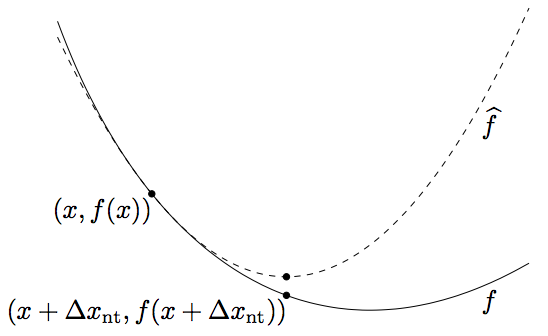
\includegraphics[width=2in]{figure/minimizer.png}
\caption{}
\end{figure}
\end{frame}

\begin{frame}
\frametitle{Interpretation II}
\framesubtitle{Steepest descent direction in Hessian norm}
    Newton step can be interpreted as 
    steepest descent method when the norm is defined as
    \be
    || u ||_{\fhess} \triangleq \sqrt{u^T \fhess u}
    \ee
\end{frame}

\begin{frame}
\frametitle{Interpretation II: Figure}
\framesubtitle{Steepest descent direction in Hessian norm}
\begin{figure}
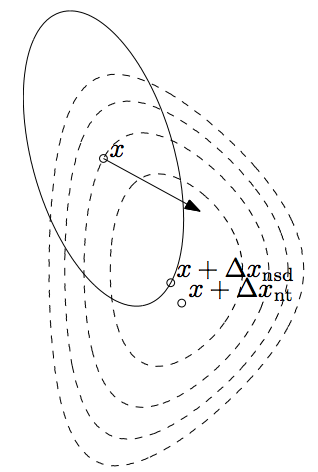
\includegraphics[width=1.3in]{figure/steepest.png}
\caption{}
\end{figure}
\end{frame}

\begin{frame}
\frametitle{Interpretation III}
\framesubtitle{Solution of linearized optimality condition}
    Newton step can also be interpreted as 
    to linear approximation over gradient $\fgrad$ around $x$.
    \be
        \nabla f(x+v) \approxeq \fgrad + \fhess
    \ee
    Set RHS to zero gives newton update.
\end{frame}

\begin{frame}
\frametitle{Interpretation III: Figure}
\framesubtitle{Solution of linearized optimality condition}
\begin{figure}
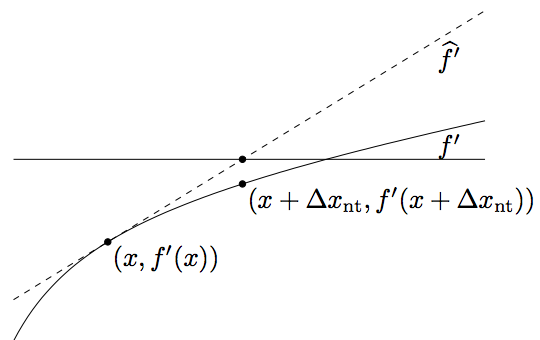
\includegraphics[width=2.2in]{figure/linear.png}
\caption{}
\end{figure}
\end{frame}

%TODO: put first-order approximation a single slide? 
% with additional analysis maybe
%\begin{frame}
%\frametitle{Another Interpretation II}
%
%\end{frame}

%%%%%%%%%%%%%%%%%%%%%%%%%%%%%%%%%%%%%%%%%%%%%%%%%%%%%%%%%%%%
%% Section TWO: Affine Invariance of Newton step
%%%%%%%%%%%%%%%%%%%%%%%%%%%%%%%%%%%%%%%%%%%%%%%%%%%%%%%%%%%%
\newcommand{\yp}{\ensuremath{y^{+}}}
\newcommand{\gradient}[3]{\ensuremath{\nabla_{#1} #2 (#3)}}
\newcommand{\hessian}[3]{\ensuremath{\nabla^2_{#1} #2 (#3)}}
\newcommand{\inv}{^{-1}}
\begin{frame}
\frametitle{Affine Invariance of Newton step}
\begin{lemma}
    Newton step is affine invariant. 
\end{lemma}

For example, let $g(y) = f(Ay)$, $\yp$ be newton update on function
$g(\cdot)$, and 
$\xp$ be newton update on function $f(\cdot)$. 
Then if $x=Ay$, we have $\xp = A\yp$.

\begin{remark}
    Affine Invariance indicates that Newton Method is vulnerable to the
    selection of coordinate system. 
\end{remark}
\begin{remark}
    Gradient Descent Method is not affine invariance. This means
    that bad coordinate choice may limit the power of Gradient Descent Method.
\end{remark}
\end{frame}

\begin{frame}
\frametitle{Proof of Affine Invariance}
    Let $x = Ay$ and $g(y) = f(Ay)$, then we have
    \be
    \hessian{y}{g}{y} &= \hessian{y}{f}{Ay} &= A^T \hessian{x}{f}{x} A \\
    \gradient{y}{g}{y} &= \gradient{y}{f}{Ay} &= A^T \gradient{x}{f}{x}
    \ee
    Newton update $\yp$ for $g(\cdot)$ can be extended as
    \be
    \yp &=& y - t(\hessian{y}{g}{y})\inv \gradient{y}{g}{y} \\
    &=& y - t(A^T \hessian{x}{f}{x} A)\inv A^T \gradient{x}{f}{x} \\
    &=& y - t\ A\inv \hessian{x}{f}{x}\inv \gradient{x}{f}{x}
    \ee
    Multiply both sides with affine tranformation $A$, 
    \be
    A\yp &=& Ay - A \cdot t\ A\inv \hessian{x}{f}{x}\inv \gradient{x}{f}{x} \\
    &=& x - t\ \hessian{x}{f}{x}\inv \gradient{x}{f}{x} \\
    &=& \xp
    \ee
\end{frame}
%%%%%%%%%%%%%%%%%%%%%%%%%%%%%%%%%%%%%%%%%%%%%%%%%%%%%%%%%%%%
%% Section three: Newton Method
%%%%%%%%%%%%%%%%%%%%%%%%%%%%%%%%%%%%%%%%%%%%%%%%%%%%%%%%%%%%

%%%%%%%%%%%%%%%%%%%%%%%%%%%%%%%%%%%%%%%%%%%%%%%%%%%%%%%%%%%%
%% Section Four: Convergence Analysis of Newton Method
%%%%%%%%%%%%%%%%%%%%%%%%%%%%%%%%%%%%%%%%%%%%%%%%%%%%%%%%%%%%
\begin{frame}
    \frametitle{Convergence Analysis: Assumption}    
    \begin{assumption}
        Let $f(\cdot)$ be the function discussed for Convergence of Newton
        Method. Both of following assumptions are what convergence analysis is
        based on.
        \begin{itemize}
            \item Function $f(\cdot)$ is strongly convex, such that
        \be
        m I \leq \fhess \leq M I
        \ee
    \item $\fhess$ is $L$-Lipschitz with constant $L > 0$, such that
        \be
        || \hessian{}{f}{y} - \hessian{}{f}{x} ||_2 \leq L ||x-y||_2,\ 
        \forall x,\ y
        \ee
        Note that induced matrix norm $|| \cdot ||_2$ equals to the largest
        singluar value of inside matrix.
        \end{itemize}
    \end{assumption}
\end{frame}

%% theorem for each phrase and implication by each phrase
\begin{frame}
    \frametitle{Convergence Analysis: Theorem}    
    \begin{theorem}[Part I]
        There exists $f,\ \eta,\ \gamma$, where $ 0 \leq \eta \leq \frac{m^2}{L}$,
        $\gamma = \frac{\alpha \beta m}{M^2}\eta^2$
        such that Newton Method with BTLS has two phrases: 
        \begin{itemize}
            \item[(a)] Global or Damped Phrase: If $||\fgrad||_2 \geq \eta$, then 
                \be
                f(\xp) - f(x) \leq -\gamma, \text{ also } 
                f(\xp) - f^* \leq c(f(x)-f^*) \label{CA:Theorem:phraseA}
                \ee
        \end{itemize}
    \end{theorem}
        Inequality \eqref{CA:Theorem:phraseA} has three implications: 
        \begin{itemize}
            \item Every newton step with BTLS gets closer to global optima by
                at least $\gamma$.
            \item Damped phrase has at most $\frac{f(x^{(0)}) -
                    f^{*}}{\gamma}$ iterations.
            \item The damped phrase essentially conforms to property of linear convergence.
        \end{itemize}
\end{frame}

\begin{frame}
    \frametitle{Convergence Analysis: Theorem}    
    \begin{theorem}[Part II]
        \begin{itemize}
            \item[(b)] Local or Quadratic Phrase: If $||\fgrad||_2 < \eta$,
                then BTLS will give $t = 1$ and we have
                \be
                \frac{L}{2m^2} ||\gradient{}{f}{\xp}||_2 \leq 
                    \bigg(\frac{L}{2m^2} ||\fgrad||_2 \bigg)^2
                \ee
        \end{itemize}
    \end{theorem}
\end{frame}

% TODO: proof of step size t = m/M satisfies the exit condition for BTLS
\begin{frame}
    \frametitle{Convergence Analysis: Proof}    
    \begin{lemma}
        $t = \frac{m}{M}$ satisfies the exit condition of BTLS.
    \end{lemma}
\end{frame}

% TODO: proof of inequality for (a) phrase and show linear convergence
% inequality
\begin{frame}
    \frametitle{Convergence Analysis: Proof}    
    \begin{lemma}
        If $||\fgrad||_2 \geq \eta$, 
        then $f(\xp) - f(x) \leq -\gamma$, 
        where  $\gamma = \frac{\alpha \beta m}{M^2}\eta^2$

    \end{lemma}
\end{frame}

% TODO: proof of inequality for (b) phrase
\begin{frame}
    \frametitle{Convergence Analysis: Proof}    
    \begin{lemma}
        If $||\fgrad||_2 < \eta$, then 
        $ \frac{L}{2m^2} ||\gradient{}{f}{\xp}||_2 \leq
                \bigg(\frac{L}{2m^2} ||\fgrad||_2 \bigg)^2 $

    \end{lemma}
\end{frame}

% TODO: proof of step size t = 1 satisfies the exit condition for BTLS
\begin{frame}
    \frametitle{Convergence Analysis: Proof}    
    \begin{lemma}
        $t = 1$ satisfies the exit condition of BTLS.
    \end{lemma}
\end{frame}
%%%%%%%%%%%%%%%%%%%%%%%%%%%%%%%%%%%%%%%%%%%%%%%%%%%%%%%%
%%%%%%%%%%%%%%%%%%%%%%%%%%%%%%%%%%%%%%%%%%%%%%%%%%%%%
\iffalse

\begin{frame}
\frametitle{Directed Graphical Models}
\begin{columns}[c]
\column{1.5in}
\includegraphics[width=1.5in]{directed_GM.pdf}
\column{1.5in}
\includegraphics[width=1.5in]{undirected_GM.pdf}
\end{columns}
$$p(\mathbf{x}) = \prod_{a \in \mathcal{V}}{p\left(x_a|x_{\text{pa}(x_a)}\right)}$$
\end{frame}


\begin{frame}
\frametitle{Directed Graphical Models}
\begin{columns}[c]
\column{1.5in}
\includegraphics[width=1.5in]{directed_GM.pdf}
\column{1.5in}
\includegraphics[width=1.5in]{undirected_GM.pdf}
\end{columns}
$$p(\mathbf{x}) = p(x_1)p(x_2|x_1)p(x_3|x_1)p(x_4|x_3)$$
%\begin{itemize}
%\item{Applications in finance, sociology, epidemiology, neuroscience and bioinformatics etc.}
%\end{itemize}
\end{frame}

\begin{frame}
\frametitle{Directed Graphical Models}
\begin{columns}[c]
\column{1.4in}
\includegraphics[width=1.4in]{directed_GM.pdf}
\column{1.4in}
\includegraphics[width=1.4in]{undirected_GM.pdf}
\end{columns}
$$p(\mathbf{x}) = p(x_1)p(x_2|x_1)p(x_3|x_1)p(x_4|x_3)$$
\begin{itemize}
\item{Applications in finance, sociology, epidemiology, neuroscience, bioinformatics...}
\end{itemize}
\end{frame}

\begin{frame}
\frametitle{Directed Graphical Models}
\begin{columns}[c]
\column{2.0in}
\centering
\includegraphics[width=1.5in]{impossibility_1.pdf}
$$p(\mathbf{x}) = p(x_1)p(x_2|x_1)p(x_3|x_2)$$
\column{2.0in}
\centering
\includegraphics[width=1.5in]{impossibility_2.pdf}
$$p(\mathbf{x}) = p(x_3)p(x_2|x_3)p(x_1|x_2)$$
\end{columns}
\begin{figure}
	\centering
		\includegraphics[width=0.40\textwidth]{intervention.pdf}
	%\caption{}
	\label{fig:2}
\end{figure}
$$\widetilde{p}(\mathbf{x}) = p(x_1)\mathbbm{1}\{x_2\}p(x_3|x_2)$$
\end{frame}


%\section{Problem Statement}
\begin{frame}
\frametitle{Time Series DAG}
\begin{figure}
	\centering
		\includegraphics[width=0.60\textwidth]{time_DAG1.pdf}
	%\caption{}
	\label{fig:2}
\end{figure}
\end{frame}

\section{Problem Statement}
\begin{frame}
\frametitle{Time Series DAG}
\begin{figure}
	\centering
		\includegraphics[width=0.60\textwidth]{time_DAG.pdf}
	%\caption{}
	\label{fig:2}
\end{figure}
\onslide<2->$$p\left(\mathbf{x}^t|\mathbf{x}^{t-1}\right) = \prod_{a \in \mathcal{V}}{p\left(x_a^{t}|x_a^{t-1}, x^{t-1}_{\text{pa}(x_a)}\right)}$$
\end{frame}

\begin{frame}
\frametitle{Directional Conditional Entropy and DAG}
\begin{itemize}
\item Want to learn parent set of each node.
\item $H(X_i|X_j)$ captures influence of $X_j$ on $X_i$.
\item Influence of  $X^{t-1}_j$ on $X^{t}_i$ is of interest in time-series DAG.
\item Conditional directional entropy: $H\left(X^t_i|X^{1,\ldots, t-1}_i, X^{1,\ldots, t}_j\right)$
\item In our setting, this reduced to $H\left(X^t_i|X^{t-1}_i, X^{t-1}_j\right)$
\end{itemize}
%\onslide<2->$$p\left(\mathbf{x}^t|\mathbf{x}^{t-1}\right) = \prod_{a \in \mathcal{V}}{p\left(x_a^{t}|x_a^{t-1}, x^{t-1}_{\text{pa}(x_a)}\right)}$$
\end{frame}



\begin{frame}
\frametitle{Algorithm}
\footnotesize
\hline
\begin{algorithmic}[1]
\STATE Input: $\left\{\mathbf{x}^t\right\}_{t=1}^{n}$.
\FOR{$a \in \mathcal{V}$} 
\STATE $\widehat{\text{pa}}(x_a) \leftarrow \phi$%, {\color{red}\text{Rej} = \phi}.
\WHILE{$\widehat{\text{pa}}(x_a)$ is growing}
\STATE $k \in \arg \min_{j \in \mathcal{V}\backslash \widehat{\text{pa}}(x_a)}\widehat{H}(x^t_a|x^{t-1}_a, x^{t-1}_{\widehat{\text{pa}}(x_a)}, {\color{red}{x^{t-1}_j}})$
\IF{$\widehat{H}(x^t_a|x^{t-1}_a, x^{t-1}_{\widehat{\text{pa}}(x_a)}, {\color{red}{x^{t-1}_j}}) < \widehat{H}(x^t_a|x^{t-1}_a, x^{t-1}_{\widehat{\text{pa}}(x_a)}) - \epsilon_2$}
\STATE $\widehat{\text{pa}}(x_a) \leftarrow \widehat{\text{pa}}(x_a) \cup \{k\}$
\ENDIF
\ENDWHILE
\ENDFOR
\end{algorithmic}
\vspace{0.1in}
\hline
\end{frame}

\begin{frame}
\frametitle{Assumptions on DAG}
%\iffalse
%\begin{figure}
%	\centering
%		%\includegraphics[width=0.75\textwidth]{}
%	\caption{}
%	\label{fig:1}
%\end{figure}
%\fi
\begin{itemize}
\item All possible transitions with positive probability $(> \gamma > 0)$.
\item For all $A \subseteq \text{pa}(i)$, $$H(x^t_i|x^{t-1}_A, x^{t-1}_i, x^{t-1}_S) - H(x^t_i|x^{t-1}_A, x^{t-1}_i, x^{t-1}_S, x^{t-1}_j) > \epsilon_2$$ for $j \in Pa(i)$ and there exists no directed path between $S$ and $i$.
%\item For any $i \in \mathcal{V}$, $$ H(x^t_i|x^{t-1}_A, x^{t-1}_i) > \epsilon' $$ for all $A \subset \mathcal{V} \backslash \{i\}$
\item For all $A \subseteq \text{pa}(i)$ and $k \in \text{pa}(\text{pa}(i))$, $$ H(x^t_i|x^{t-1}_A, x^{t-1}_k) - H(x^t_i|x^{t-1}_A, x^{t-2}_k) > \epsilon_1 $$ for all $A \subset \mathcal{V} \backslash \{i\}$
\end{itemize}
\end{frame}

\begin{frame}
\frametitle{Grandparent Effect}
\footnotesize
\begin{figure}
	\centering
		\includegraphics[width=0.45\textwidth]{diamond.png}
	%\caption{}
	%\label{fig:2}
\end{figure}
$$p\left(x^{t}_{i}|x^{t-1}_{i}, x^{t-1}_{\text{pa}(x_i)}\right) = f(x^{t-1}_{i}, x^{t-1}_{\text{pa}(x_i)}) = g(x^{t-1}_{i}, x^{t-2}_k)$$
\begin{itemize}
\item If $x^{\cdot}_k$ is highly correlated across time, algorithm may pick $x_k$ as a member of pa$(x_i)$.
\item Trace one step back and use the fact that $x^{t-1}_k = h(x_k^{t-2},\ldots)$.
\end{itemize}
\end{frame}

\begin{frame}
\frametitle{Algorithm}
\footnotesize
\hline
\begin{algorithmic}[1]
\STATE Input: $\left\{\mathbf{x}^t\right\}_{t=1}^{n}$.
\FOR{$a \in \mathcal{V}$} 
\STATE $\widehat{\text{pa}}(x_a) \leftarrow \phi$%, {\color{red}\text{Rej} = \phi}.
\WHILE{$\widehat{\text{pa}}(x_a)$ is growing}
\STATE {\tiny{{\color{blue}{$\mathcal{U} = \left\{j \in \mathcal{V}\backslash \{\widehat{\text{pa}}(x_a) \cup \{a\}\}:\widehat{H}(x^t_a|x^{t-1}_a, x^{t-1}_{\widehat{\text{pa}}(x_a)}, {\color{red}{x^{t-1}_j}})  <  \widehat{H}(x^t_a|x^{t-1}_a, x^{t-1}_{\widehat{\text{pa}}(x_a)},{\color{red}{x^{t-2}_j}})  - \epsilon_1\right\}$}}}}
\STATE $k \in \arg \min_{{\color{blue}{j \in \mathcal{U}}}}\widehat{H}(x^t_a|x^{t-1}_a, x^{t-1}_{\widehat{\text{pa}}(x_a)}, {\color{red}{x^{t-1}_j}})$
\IF{$\widehat{H}(x^t_a|x^{t-1}_a, x^{t-1}_{\widehat{\text{pa}}(x_a)}, {\color{red}{x^{t-1}_j}}) < \widehat{H}(x^t_a|x^{t-1}_a, x^{t-1}_{\widehat{\text{pa}}(x_a)}) - \epsilon_2$}
\STATE $\widehat{\text{pa}}(x_a) \leftarrow \widehat{\text{pa}}(x_a) \cup \{k\}$
\ENDIF
\ENDWHILE
\ENDFOR
\end{algorithmic}
\vspace{0.1in}
\hline
\end{frame}


\begin{frame}
\frametitle{Why does this work with enough samples}
\footnotesize
\begin{itemize}
\item Define 
$$\left\|P - \widehat{P}\right\|_1 = \sum_{x \in \mathcal{X}}\left|P(x) - \widehat{P}(x)\right|$$
\item We have
$$\left\|H(P) - H(\widehat{P})\right\|_1 \leq -\left\|P - \widehat{P}\right\|_1\log \frac{\left\|P - \widehat{P}\right\|_1}{\left| \mathcal{X}\right|}$$
\end{itemize}
\begin{theorem}\textbf{Concentration Result for Markov Chains:}
Let $X$ be a Markov Chain and $T$ be its $\delta-$mixing time $(\delta < 1/8)$. Let $X_1,\ldots, X_n$ be $n$ step random walk on $X$. Define $Z = \sum_{t=1}^{n}f(X_t)$. For $\delta \in [0,1]$ we have
$$\mathbb{P}[Z \geq (1+\epsilon)\mu n] \leq C(\pi_{1})\exp \left(-\epsilon^{2}\mu n/(72T)\right)$$
and
$$\mathbb{P}[Z \leq (1-\epsilon)\mu n] \leq C(\pi_{1})\exp \left(-\epsilon^{2}\mu n/(72T)\right)$$
\end{theorem}
\end{frame}

\section{Simulation Results}
\begin{frame}
\frametitle{Line graph}
\begin{figure}
	\centering
		\includegraphics[width=0.75\textwidth]{line_graph.png}
	%\caption{}
	%\label{fig:2}
\end{figure}
\end{frame}

\begin{frame}
\frametitle{Line graph with Loop}
\begin{figure}
	\centering
		\includegraphics[width=0.70\textwidth]{line_loop.png}
	%\caption{}
	%\label{fig:2}
\end{figure}
\end{frame}

\begin{frame}
\frametitle{Tree graph}
\begin{figure}
	\centering
		\includegraphics[width=0.70\textwidth]{tree_graph.png}
	%\caption{}
	%\label{fig:2}
\end{figure}
\end{frame}
%%%%%%%%%%%%%%%%%%%%%%%%%%%%%%%%%%%%%%%%%%%%%%%%%%%%%%%%%%%%%%%%%%
%%%%%%%%%%%%%%%%%%%%%%%%%%%%%%%%%%%%%%%%%%%%%%%%%%%%%%%%%%%%%%%%%
\fi

\end{document}
